\documentclass[relatorio.tex]{subfiles}
\begin{document}
Nesta última fase proposta pelo enunciado do trabalho prático foi necessário a 
criação de novas classes, sendo estas acrescentadas com base na estrutura realizada
na primeira fase. As novas classes foram criadas com base nos novos elementos do ficheiro
XML, nomeadamente, \textit{texture}, \textit{color} e \textit{lights}, mantendo assim a 
responsabilidade de leitura do XML para a classe responsável por manipular estes elementos.

Apesar de não existir \textit{normals} no ficheiro XML, foi criada a classe \textit{normals},
responsável pela leitura das normais presentes no ficheiro .3d criado pelo \textit{generator}.

\begin{landscape}
    \begin{figure}
        \centering
        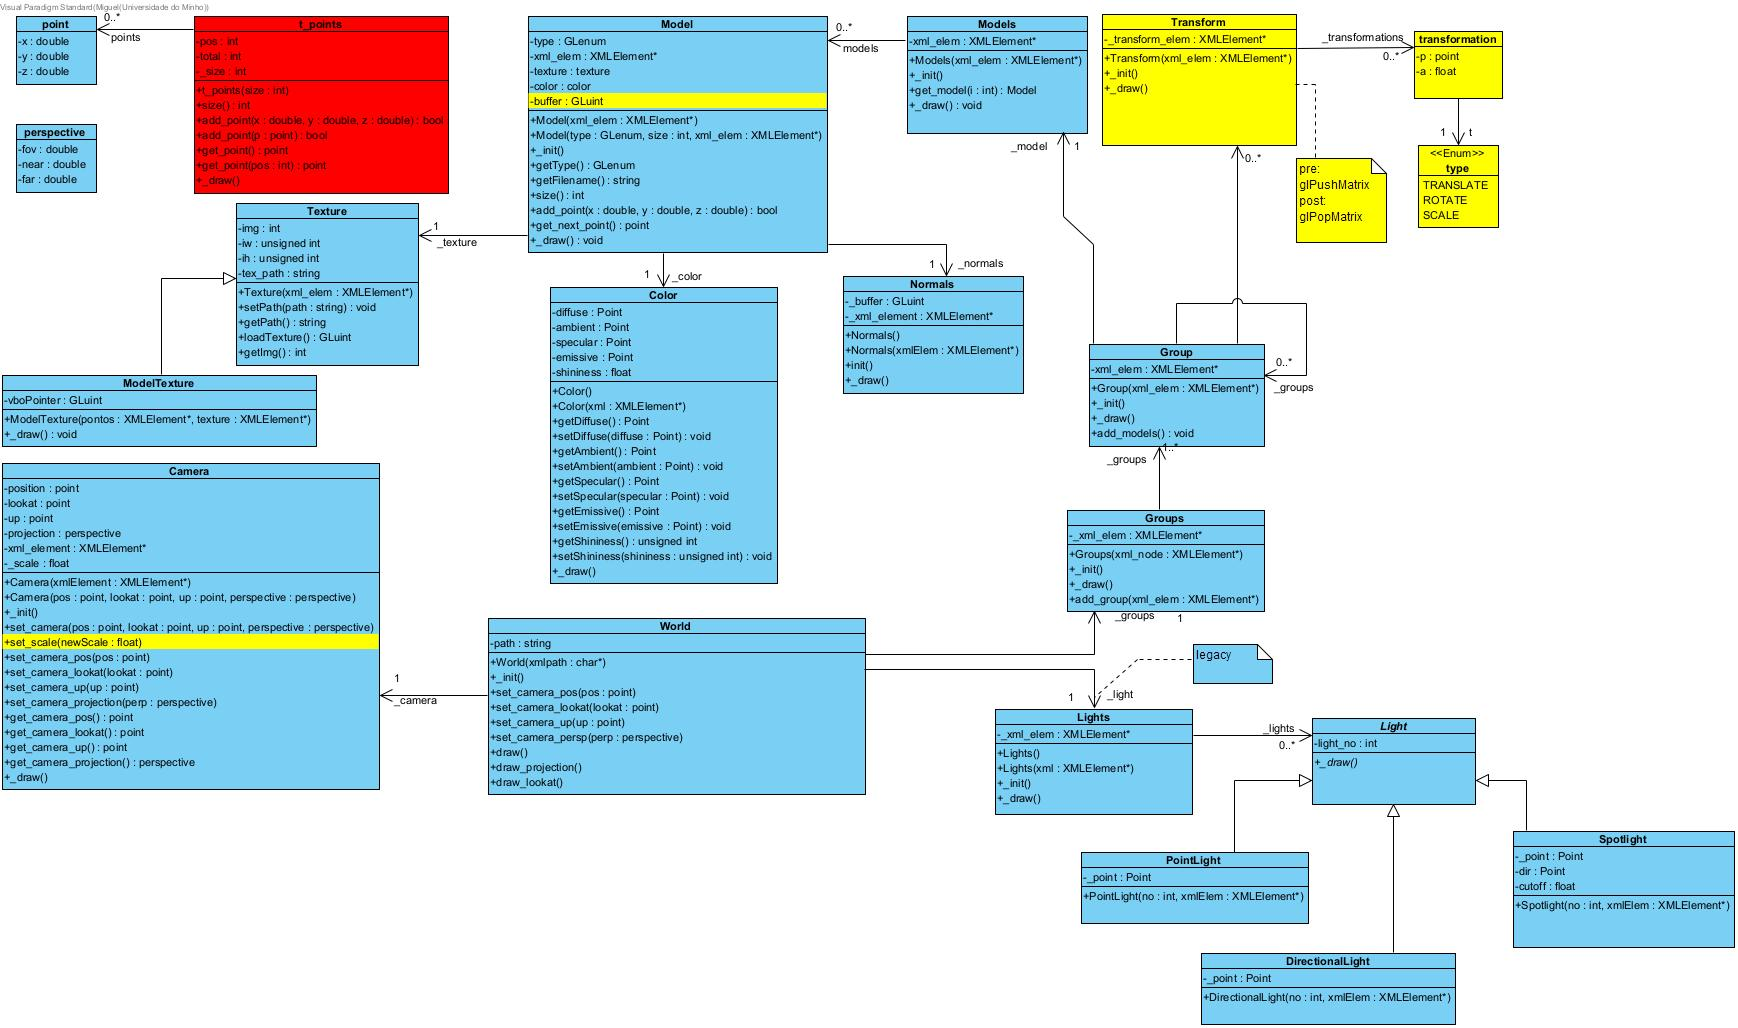
\includegraphics[width=\linewidth]{assets/classe.jpg}
        \caption{Diagrama de classes} \label{fig:dig_classes}
    \end{figure}
\end{landscape}

\subsection{Luzes}

\subsection{Cores}
A classe \textit{Color} tem como argumentos as 5 componentes da luz,
que são inicializadas por defeito com os valores passados pela equipa docente
no enunciado do trabalho. 

\subsection{Texturas}
Para tratar das Texturas foram criadas 2 classes, uma superclasse
\textit{Texture} e a sua subclasse \textit{ModelTexture}.

Na classe \textit{Texture} é onde é feito o processamento da imagem com a textura
a partir da função \textit{loadTexture}. Esta utiliza como parâmetros de
\textit{wrap} o \textit{repeat} tanto em S como em T. De maneira a obter
uma textura com melhor qualidade e ainda melhorar o desempenho foi utilizado
o \textit{MipMapping}, fazendo proveito da primitiva \textit{linear} tanto para a 
escolha do \textit{pixel} como também da textura e assim evitar obter um resultado pixelizado.

A classe \textit{ModelTexture} por sua vez é responsável por processar as coordenadas de texturas
recebidas no ficheiro ".3d", colocando-as no \textit{buffer}.

\end{document}
